\subsubsection{Recursius}

La recursió és una tècnica la qual empra una funció recursiva, aquesta funció consta de dues parts:

\begin{itemize}
\item Cas base -> finalitza la recursió.
\item Cas recursiu -> continua la recursió (crida la funció recursiva).
\end{itemize}

La recursió ens l'hem d'imaginar com un arbre en el qual cada crida recursiva forma una nova branca d'aquest i s'allarga fins que arriba a un cas base. \newline

De nou, posaré l'exemple de la seqüència de Fibonacci per comparar la recursió amb la iteració. \newline

La formula a utilitzar és la mateixa que la que hem utilitzat en la recursió. \newline

fib_n =
\begin{cases}
0 & \text{si $n = 0$}\\
1 & \text{si $n = 1$}\\
fib_{n-1}+fib_{n-2}& \text{si $n \geq 2$}
\end{cases} \newline \newline

Els primers dos casos: $n = 0$ i $n = 1$, seran els casos base. \newline

L'últim cas: $n \geq 2$, serà el cas recursiu. \newline

Donada qualsevol $n$ tal que la $n-esima$ posició en la seqüència de Fibonacci, amb l'ús de la recursió podem trobar $fib_n$ amb una complexitat de $O(2^n)$.

Cal recalcar que podem fer-ho també amb una complexitat de $O(n)$, però requereix l'ús de la programació dinàmica. \newline

\begin{lstlisting}
int fib(int n){

    if (n == 0) // primer cas base
        return 0;

    if (n == 1) // segon cas base
        return 1;

    return fib(n - 1) + fib(n - 2); // cas recursiu
}

int main(){
    cout << "Introdueix n: " << endl;
    int n; // Input -> 9
    cin >> n;
    cout << fib(n); // Output -> 34
}
\end{lstlisting}


\begin{center}
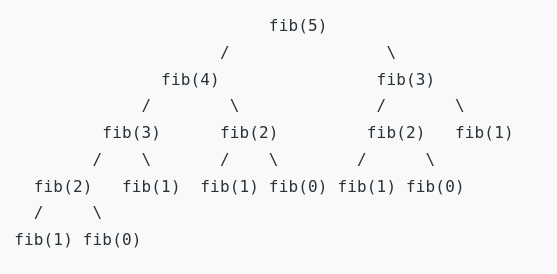
\includegraphics[width=.9 \textwidth]{crides.png}

\caption{\emph{Figura 3: Crides recursives fibonacci. Font: \url{https://www.geeksforgeeks.org/program-for-nth-fibonacci-number/}}}
\end{center}

A la figura 3, podem analitzar totes les crides recursives que es realitzen amb $n = 5$.

Podem observar que hi ha crides repetides i que es poden optimitzar per no haver de recalcular-les de forma estúpida, aquestes optimitzacions es poden dur a terme com he dit anteriorment, amb la programació dinàmica. \newline

A la figura 3, considerem que la branca de fib(3) i fib(2) està repetida.